\documentclass[11pt]{beamer}
\usetheme{Antibes}
\defbeamertemplate{description item}{align left}{\insertdescriptionitem\hfill}
\usepackage{ragged2e}
\graphicspath{{./img/}}
\usepackage {tikz}
\usetikzlibrary{positioning}
\definecolor {processblue}{cmyk}{0.96,0,0,0}
\title{FTech Training}
\subtitle{Using Beamer}
\author{Luc Nguyen}
\institute{HUST}
\date{\today}
\usetheme{Boadilla}
\begin{document} % auto-compile by Ctrl + S
	\begin{frame}
		\frametitle{\textbf{CONVOLUTIONAL NEURAL NETWORK}}
		\framesubtitle{OUTLINE}
		\begin{itemize}
			\item Basic concepts
			\item Convolutional Neural Network History
			\item Convolutional Neural Network Architectures 
			\item Applications
		\end{itemize}
	\end{frame}
	\begin{frame}
		\frametitle{\textbf{CONVOLUTIONAL NEURAL NETWORK}}
		\framesubtitle{Basic concepts}
		\setbeamertemplate{description item}[align left]
		\begin{minipage}{0.57\textwidth}
			\begin{description}
				\item[Neural network]A network or a ciucuit of neurons
				\item[Artificial neural networks(ANN)]computing systems insipred by biological neural network that constitute animal brain
			\end{description}
		\end{minipage}
		\begin{minipage}{0.4\textwidth}
			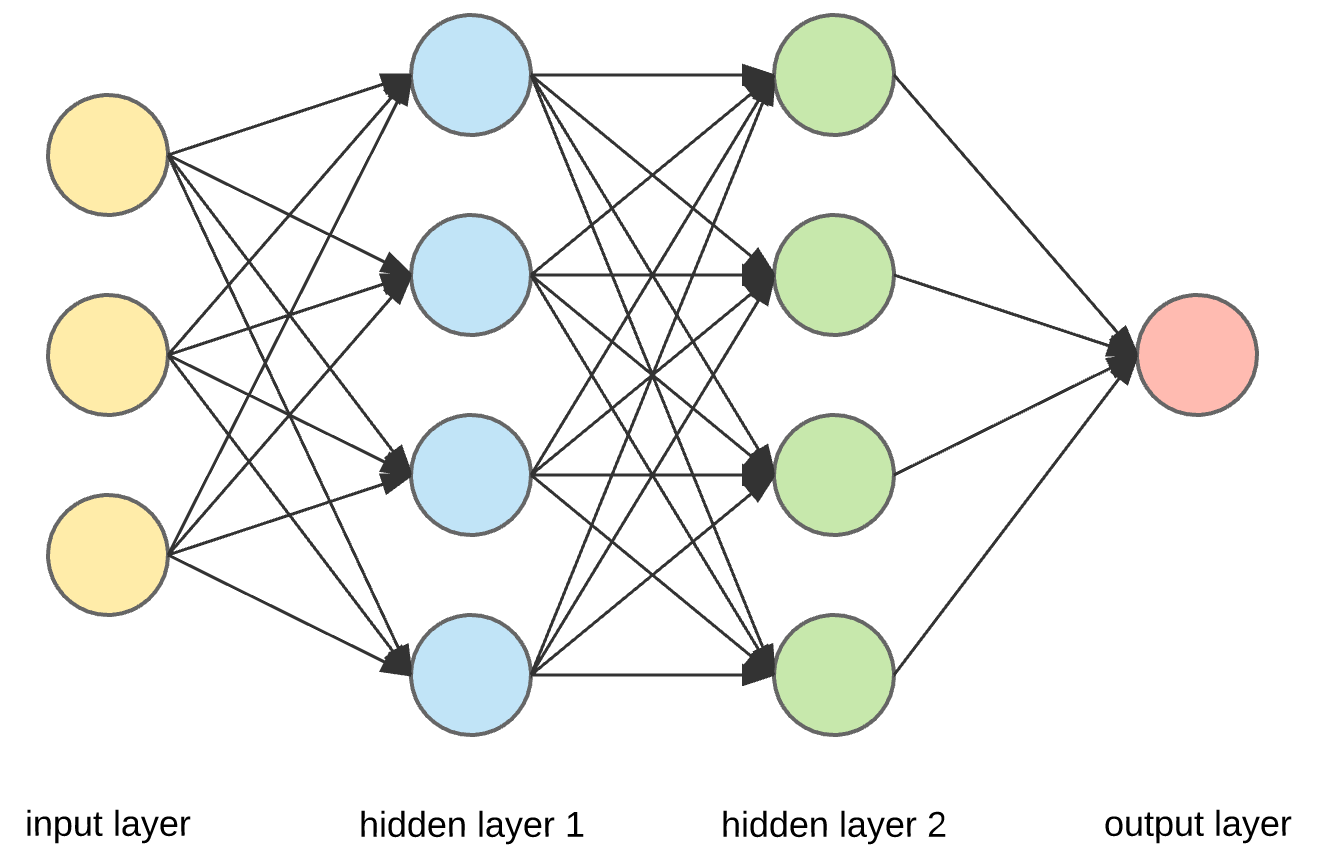
\includegraphics[scale=0.12]{CNN_Visualize.png}
		\end{minipage}
		
		\begin{description} 
			\item[Node (Perceptron)] A computational unit that has one or more weighted input connections
			\item[Layers] Sets of neurons
			\item[Shallow learning] Neural network with 1 hidden layer
			\item[Deep learning] Neural network with more than 1 hidden layer
		\end{description}
	\end{frame}
	\begin{frame}
		\frametitle{\textbf{CONVOLUTIONAL NEURAL NETWORK}}
		\framesubtitle{Convolutional Neural Network History}  % HISTORY
		\textbf{Convolutional neural network : }   is a class of deep neural networks, most commonly applied to analyzing visual imagery %Artificial neural networks where the connections between layers appear to be somewhat arbitrary
		\begin{minipage}{0.5\textwidth}
			\begin{itemize}
				\item \textbf{LeNet} (Yann LeCun, 1989), LeNet-5 (Yann LeCun, 1998)
				\item \textbf{Max pooling:} 1990, Yamaguchi
				\item \textbf{AlexNet} : 2012
				\item \textbf{ZFNet} : 2013
				\item \textbf{VGGNet} : 2014
				\item \textbf{GoogleNet, ResNets} : 2015
				\item \textbf{Densenet} : 2016
			\end{itemize}
		\end{minipage}
		\begin{minipage}{0.4\textwidth}
			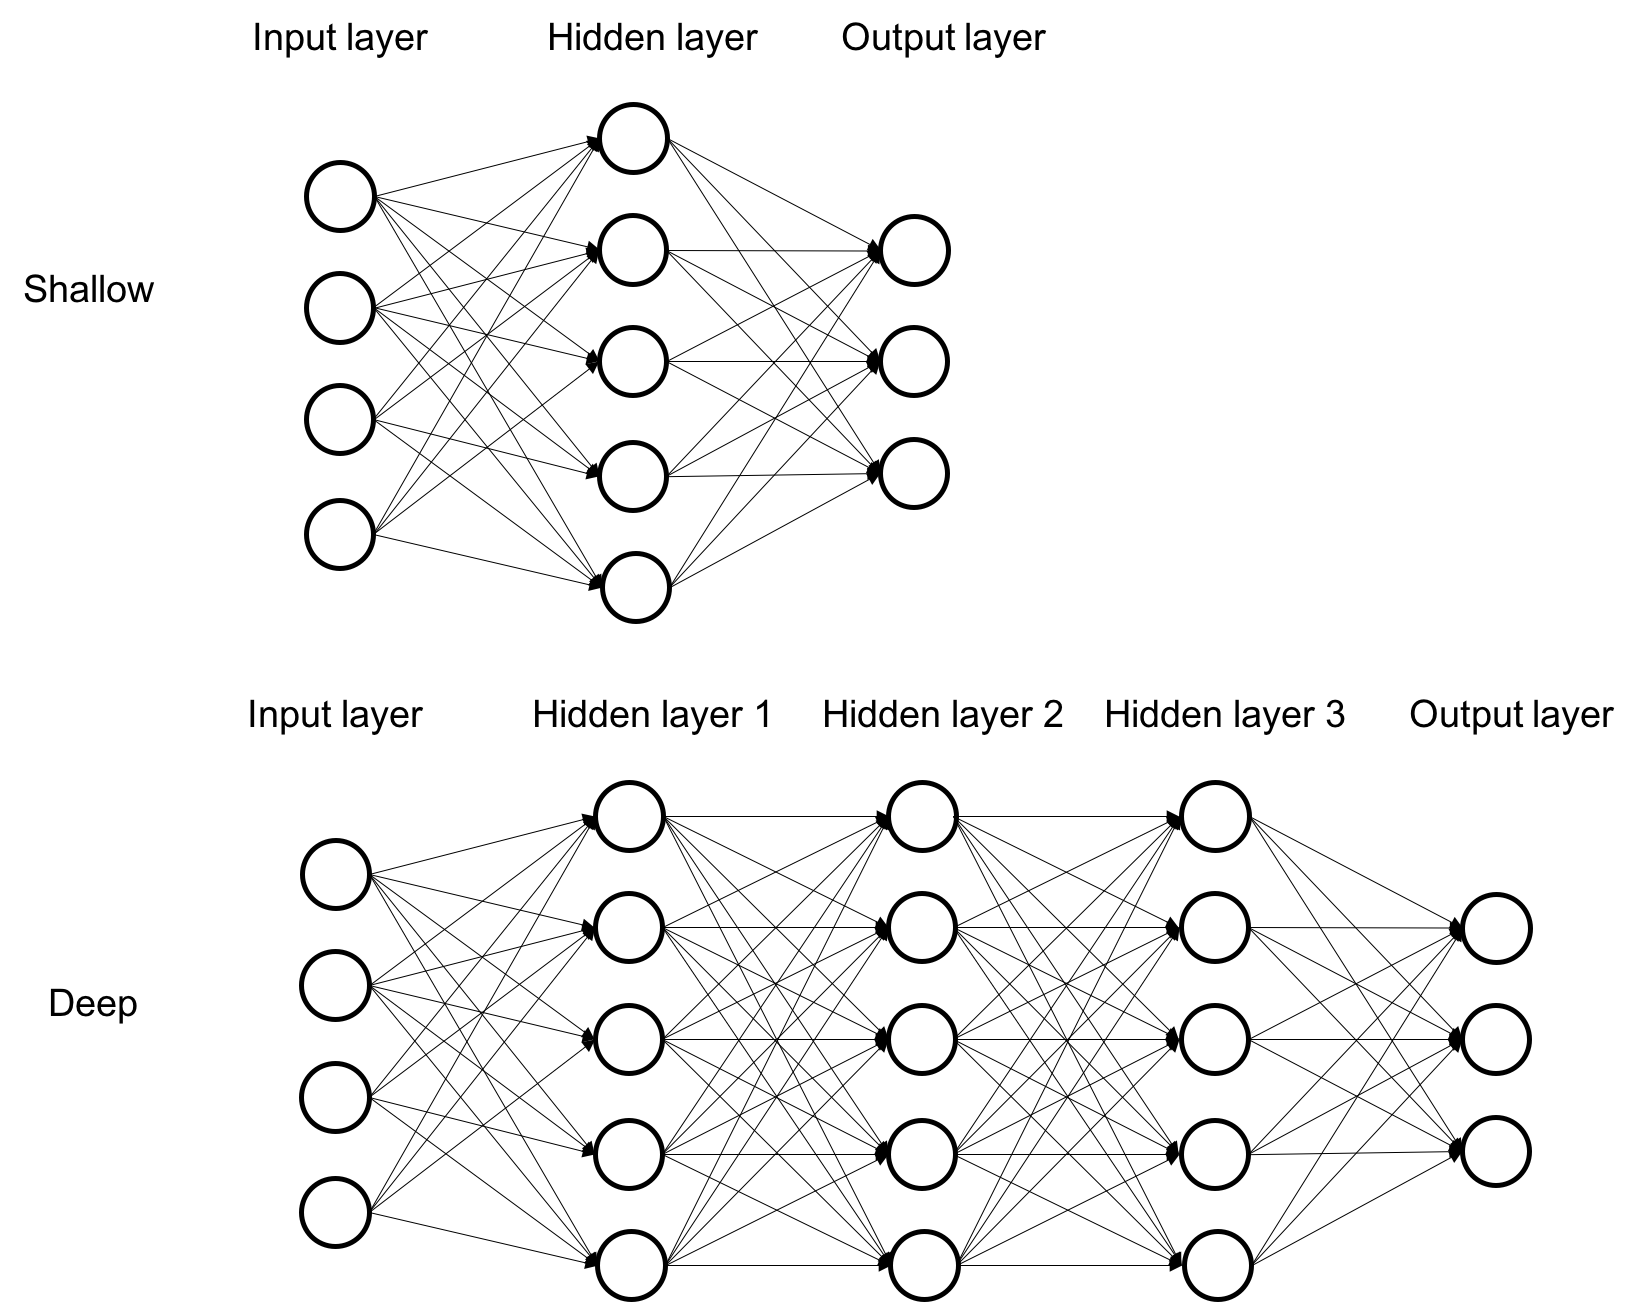
\includegraphics[scale=0.2]{shallow_deep_learning.png}
		\end{minipage}
	\end{frame}
	\begin{frame}
		\frametitle{\textbf{CONVOLUTIONAL NEURAL NETWORK}}
		\framesubtitle{Convolutional Neural Network Architectures}
		\begin{figure}[h!]
			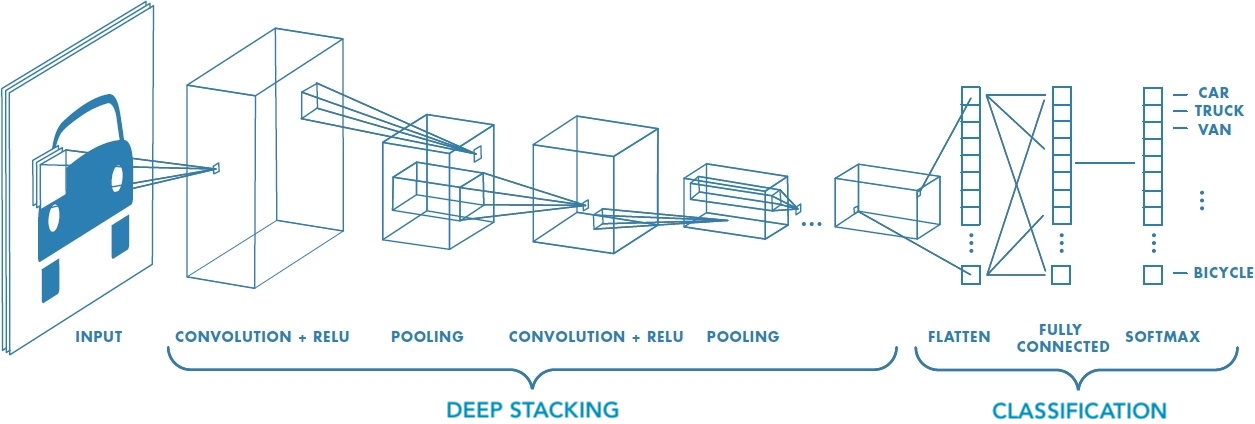
\includegraphics[width=0.65\textwidth]{CNN_Layers.png}
			\caption{A Generality of Convolutional Neural Network Architectures}
		\end{figure}
		\begin{figure}[h!]
			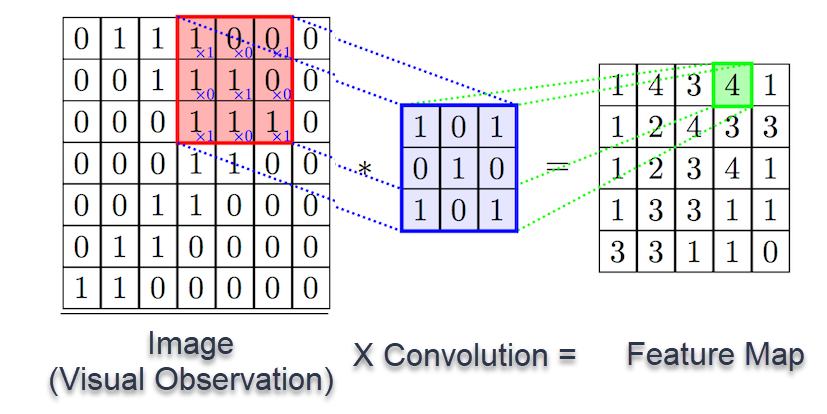
\includegraphics[width=0.5\textwidth]{cnn_conv.png}
			\caption{Visualization of Convolution}
		\end{figure}
		{Comparison to a regular neural network architectures} 
	\end{frame}
	\begin{frame}
		\frametitle{\textbf{CONVOLUTIONAL NEURAL NETWORK}}
		\framesubtitle{Convolutional Neural Network Architectures}
		\textbf{Other techniques}

		\begin{itemize}
			\begin{minipage}{0.45\textwidth}
				\item Pooling: 
				\begin{figure}[h!]
					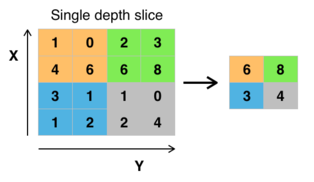
\includegraphics[width=0.8\textwidth]{Max_pooling.png}
					\caption{Max pooling}
				\end{figure}
			\end{minipage}
			\begin{minipage}{0.45\textwidth}
				\item Dropout: 
				\begin{figure}[h!]
					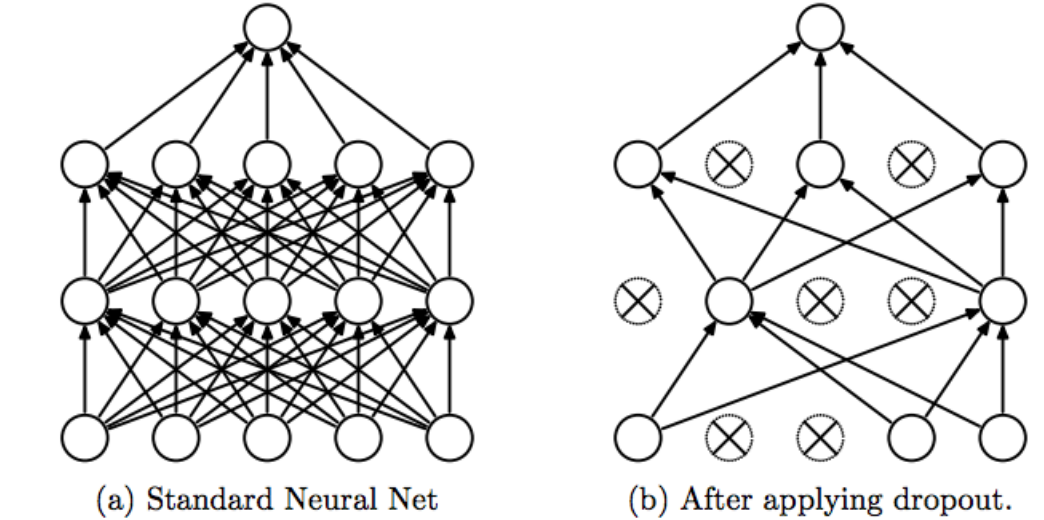
\includegraphics[width=0.8\textwidth]{dropout.png}
					\caption{Dropout}
				\end{figure}
			\end{minipage}
			\begin{minipage}{0.45\textwidth}
				\item Local Contrast Normalization: 
				\begin{figure}[h!]
					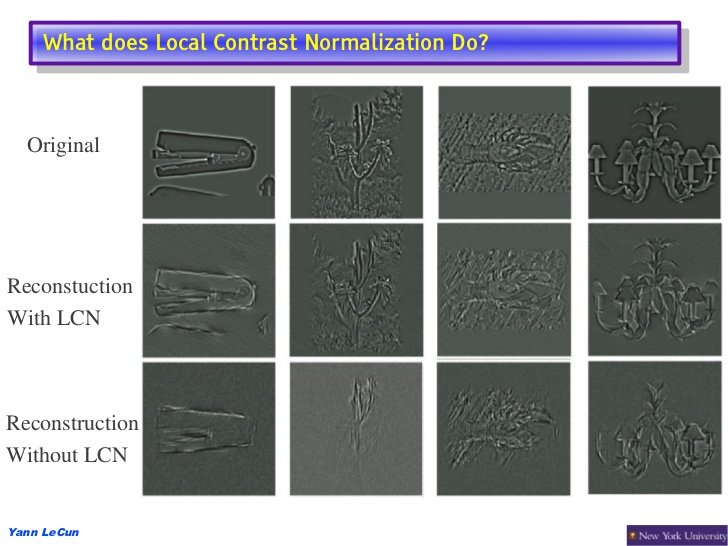
\includegraphics[width=0.7\textwidth]{LCN.jpg}
					\caption{Local Contrast Normalization}
				\end{figure}
			\end{minipage}
			\begin{minipage}{0.45\textwidth}
				\item Backpropagation
				\item Stochastic Gradient Descent
				\item Learning Rate Decay
				\item Long Short-Term Memory
			\end{minipage}
		\end{itemize}
	\end{frame}
	\begin{frame}
		\frametitle{\textbf{CONVOLUTIONAL NEURAL NETWORK}}
		\framesubtitle{Convolutional Neural Network Architectures}
		\begin{itemize}
			\item \textbf{Advantages:}
			\begin{itemize}
				\item Simplify computation to a great extent without losing the essence of the data
				\item Great at handling image classification
			\end{itemize}
			\item \textbf{Disadvantages:}
			\begin{itemize}
				\item Slow to train on a old GPU
				\item Need pre-processing (hand-engineered)
				\item CNN do not encode the position and orientation of the object
				\item Lack of ability to be spatially invariant
			\end{itemize}
		\end{itemize}
	\end{frame}
	\begin{frame}
		\frametitle{\textbf{CONVOLUTIONAL NEURAL NETWORK}}
		\framesubtitle{Applications} % APPLICATIONS
		\begin{figure}[h!]
			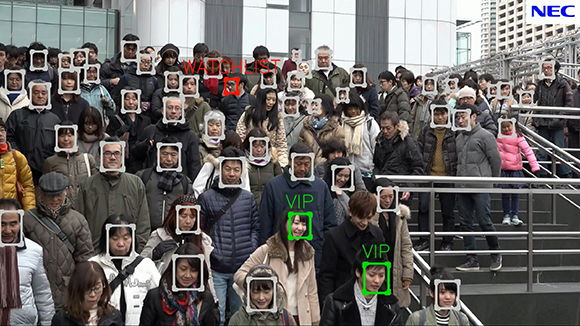
\includegraphics[width=0.4\textwidth]{ImgAndVidRecog1.jpg}
			\caption{Image and video recognition}
		\end{figure}
		\begin{figure}[h!]
			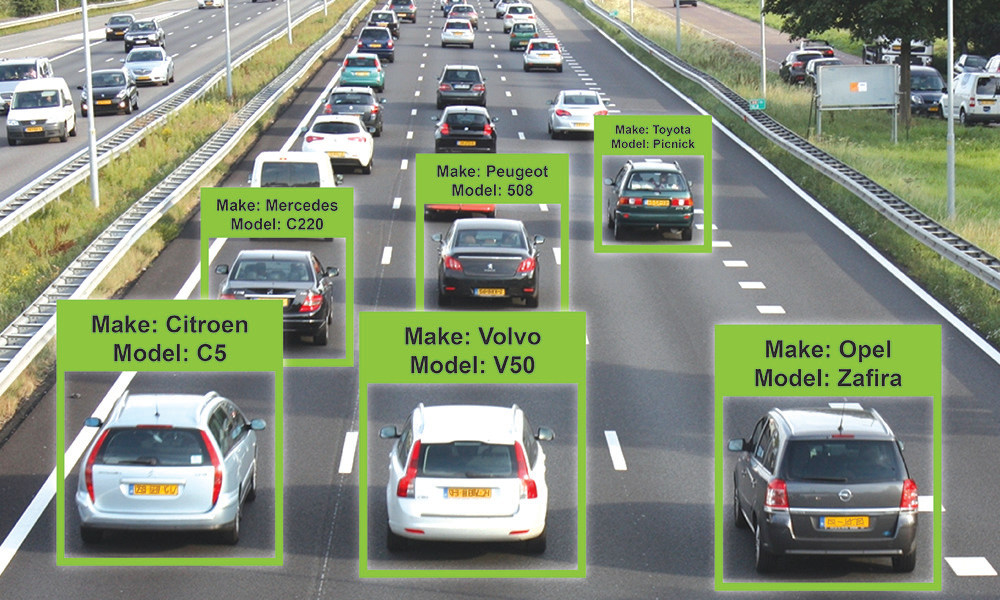
\includegraphics[width=0.4\textwidth]{ImgAndVidRecog2.jpg}
			\caption{Recommendation system}
		\end{figure}
	\end{frame}
	\begin{frame}
		\begin{figure}[h!]
			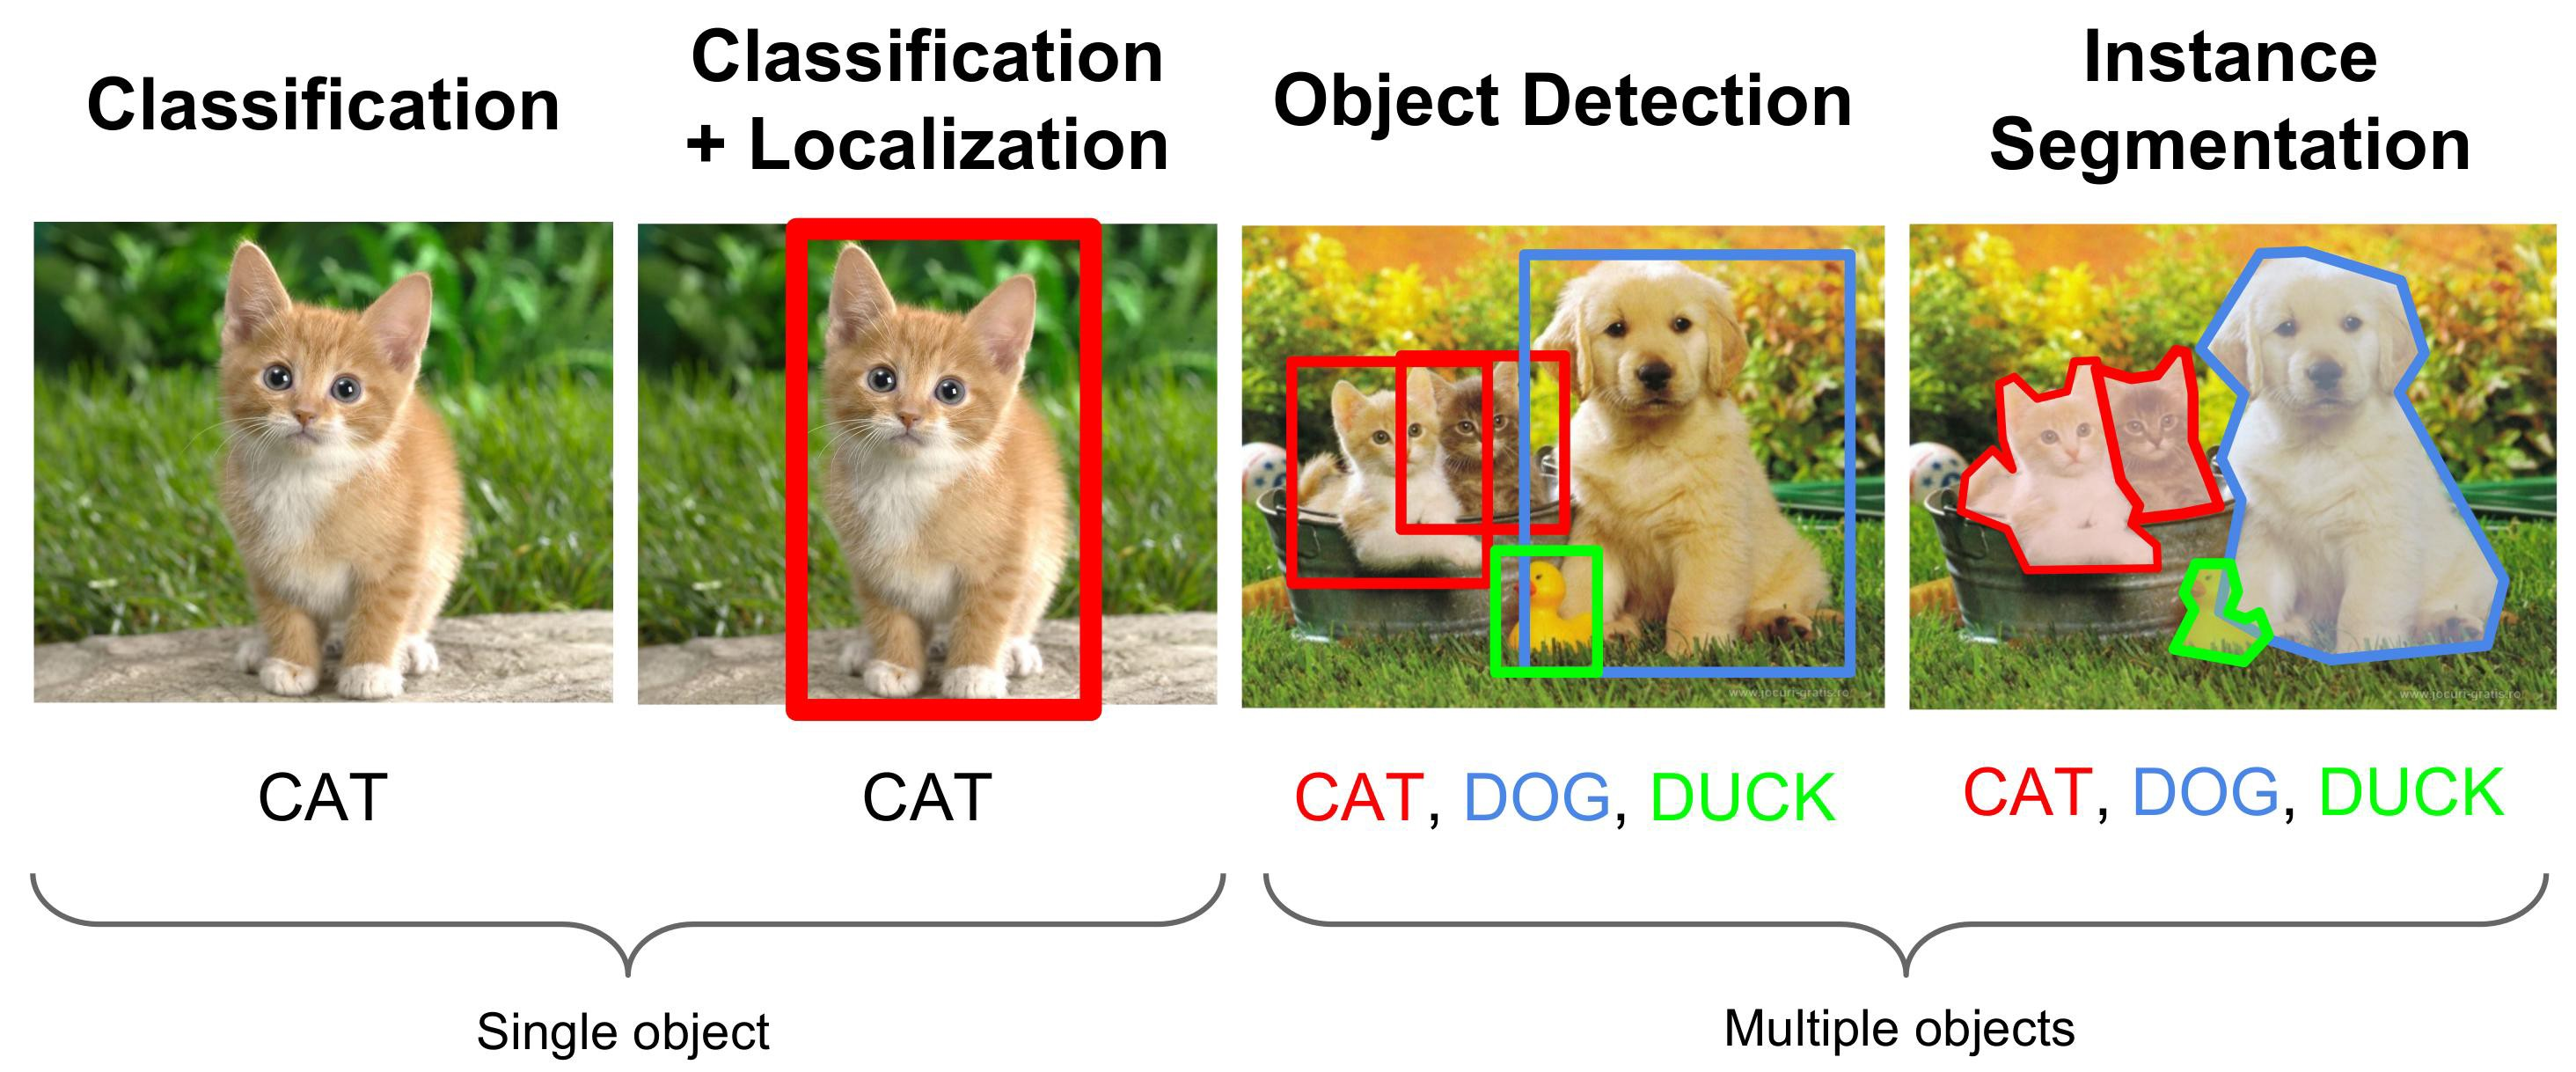
\includegraphics[width=0.4\textwidth]{img_classify.jpeg}
			\caption{Image classification}
		\end{figure}
		\begin{figure}[h!]
			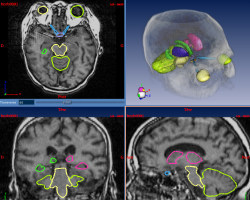
\includegraphics[width=0.4\textwidth]{medical_analysis.jpg}
			\caption{Medical image analysis}
		\end{figure}
	\end{frame}
	
\end{document} 